\subsubsection*{PowerStack}

\paragraph{Overview} 
Power remains a critical constraint for Exascale. As we design supercomputers at larger scales, power becomes an expensive and limited resource. Inefficient management of power leads to added operational costs as well as low scientific throughput. Although hardware advances will contribute a certain amount towards achieving high energy efficiency, they will not be sufficient, creating a need for a sophisticated system software approach. Significant advances in software technologies are thus required to ensure that Exascale systems achieve high performance with effective utilization of available power. Distributing available power to nodes while adhering to system, job and node constraints involves complex decision making in software. 

The ECP PowerStack sub-area in Argo explores hierarchical interfaces for power management at three specific levels: batch job schedulers, job-level runtime systems, and node-level managers. Each level will provide options for adaptive management depending on requirements of the supercomputing site under consideration. Site-specific requirements such as cluster-level power bounds, user fairness, or job priorities will be translated as inputs to the job scheduler. The job scheduler will choose power-aware scheduling plugins to ensure compliance, with the primary responsibility being management of allocations across multiple users and diverse workloads. Such allocations (physical nodes and job-level power bounds) will serve as inputs to a fine-grained, job-level runtime system to manage specific application ranks, in-turn relying on vendor-agnostic node-level measurement and control mechanisms. The figure below presents an overview of the envisioned PowerStack, which takes a holistic approach to power management.  Additionally, power monitoring and management support for science workflows (such as MuMMI Cancer workflow) and in-situ visualization workflows is being developed. Furthermore, solutions for co-scheduling challenges for extremely heterogeneous architectures are being designed as a part of a university subcontract to University of Arizona. 

This project is essential for ECP because it enables Exascale applications to operate safely with optimal performance under power and energy constraints. This project is also essential for building a sophisticated hierarchical software stack proposed by the ECP ATDM (LLNL) and Flux projects. Additionally, the project fulfills an essential need for ECP by enabling vendor and academic collaborations that provide for accelerated adoption of best practices and better interoperability at scale. By leveraging the software developed in this project, compute centers can safely operate under power and energy constraints while maximizing performance and scientific throughput. 

\begin{figure}[t]
	\centering
	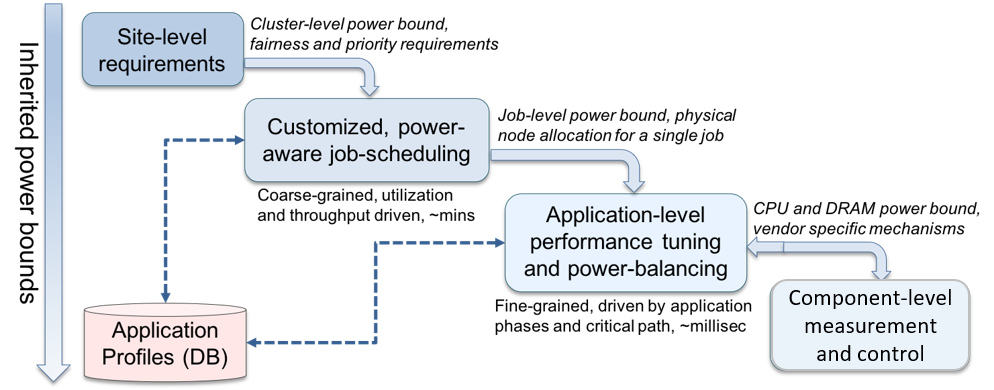
\includegraphics[scale = 0.7]{projects/2.3.1-PMR/2.3.1.19-Argo-PowerSteering/PowerStack_v2.png}
	\caption{Envisioned PowerStack}
	\label{fig:pstack}
\end{figure}


\paragraph{Key Challenges}
Power management in software is challenging due to the dynamic phase behavior of applications, processor manufacturing variability, and the increasing heterogeneity of node-level components. While several scattered research efforts exist, a majority of these efforts are site-specific, require substantial programmer effort, and often result in suboptimal application performance and system throughput. Additionally, these approaches are not production-ready and are not designed to cooperate in an integrated manner. A holistic, generalizable and extensible approach is still missing in the HPC community, and a goal for the ECP PowerSteering project is to provide a solution for this technology gap. 

Another set of challenges come from portability issues. Existing solutions are targeted toward specific Intel microarchitectures as well as programming models. Additionally, some of the existing solutions  violate the specified power budget before reaching a steady state, resulting in power fluctuations as well as unsafe operation. As part of this project, we strive to provide portability as well as safe operation using both hardware-level and application-level information for adaptive configuration selection and critical path analysis.

\paragraph{Solution Strategy}
As discussed earlier, our solution is to develop an end-to-end deployable stack, that combines coarse-grained power-scheduling (Flux, SLURM) with fine-grained job-level runtime system (Intel GEOPM) while ensuring vendor neutrality. Such a stack can operate transparently to user applications.  At the scheduler level, we are working on extending SLURM and Flux resource managers to be power-aware. Here, we are looking at both static, coarse-grained power management as well as portability through SPANK plugins. For the \emph{job-level}, a power management runtime system called GEOPM that will optimize performance of Exascale scientific applications transparently under power and/or energy constraints is being developed in collaboration with Intel. At the node-level, vendor-neutral interfaces are being developed as part of variorum library, to allow for support for Intel, IBM, AMD, ARM, and HPE/Cray platforms.  In order to accomplish portability and smooth integration, we are closely collaborating with ECP MuMMI workflow project and ECP Flux projects, and with University of Arizona. We are actively engaging ECP users in order to support power management in a non-intrusive and transparent manner. 

\paragraph{Recent Progress}
We achieved three milestones in September 2019. The first was to finish development of GRM (Flux and SLURM Spank plugin), delivered as part of ECP Argo. Here, we developed a SPANK plugin in SLURM to allow for power management across jobs -- we chose the SPANK plugin due to its portability benefits and non-dependence on specific SLURM versions. We also released a variation-aware scheduling plugin for Flux, which involved mitigating variation resulting from manufacturing differences under power caps on large-scale clusters. 

The other two milestones were delivered as part of PowerSteering project which merged with Argo for FY20. Here, we worked on GEOPM integration on non-intel architecture, and for evaluation of power-aware mappers in the Legion runtime system framework. We chose IBM Power9 (Witherspoon) architecture for GEOPM, which applies well to the Sierra/Summit systems. We developed a DVFS-based model for Intel GEOPM and leveraged GPU NVIDIA's NVML library to create this port.  The second milestone involved developing a new power-aware mapper in Legion and creating a two benchmarks for evaluation. This allowed for support of power management tools for non-MPI applications. Releases were made separately for the two milestones on GitHub, and were evaluated on an isolated IBM P9 node (alehouse) and quartz cluster (2K nodes) at LLNL. 

We established the PowerStack community charter in June 2018, involving collaborators across multiple vendors (Intel, IBM, ARM, HPE, AMD), academic institutions (TU Munich, Univ. Tokyo, Univ. Bologna, Univ. Arizona), and national laboratories (Argonne National Lab).The goal for this team is to design a holistic, flexible and extensible concept of a software stack ecosystem for power management. Over the past 1.5 years, this group is looking at engineering and research challenges, along with RFP/procurement designs through active vendor interaction and involvement. A face-to-face seminar will be held the week prior to SC19 from November 13-15, 2019 in Colorado Springs for the same, the details of which can be found here: \url{https://hpcpowerstack.github.io/powerstack-nov19.html}. 

\paragraph{Next Steps}
We will continue our research and development work as planned toward the FY20 milestones. More specifically, we will continue development for variorum library, extend Intel GEOPM's new codebase, continue development of scheduler components such as Flux and SLURM, work on GPU power capping research, and enable user-space access to power management on diverse architectures. We will also explore co-scheduling challenges in power management (University of Arizona) and development of power monitoring and control tools for science workflows such as MuMMI cancer workflow and in-situ visualization workflows. We will also deploy components across Tri-labs through the TOSS operating system environment, 

